\section{Related Work}
\label{sec:Related Work}

\subsection{Text-to-Image Models} 
The method of generating images from given textual descriptions has been extensively explored. GAN-based works have demonstrated impressive capabilities in producing realistic images~\cite{tao2022df,xu2018attngan,zhang2021cross}. Generative transformer methods usually train large-scale autoregressive transformers in a discrete token space to model the generation process~\cite{ramesh2021zero,yu2022scaling,yu2023scaling}. More recently, diffusion models have been applied in text-to-image tasks, achieving state-of-the-art results in generating high-fidelity images~\cite{rombach2022high,podell2023sdxl,esser2024scaling}. Given a text prompt, the model typically converts the text into a latent vector with the help of a pretrained language model~\cite{radford2021learning}, and then generates images from pure Gaussian noise through a iterative denoising process. Although these models have demonstrated remarkable capabilities in image generation, they struggle to ensure that the generated images perform well across multiple aesthetic dimensions.



% \subsection{Fine-Tuning Text-to-Image Models} 
% Given a pre-trained text-to-image model, we can adapt it to a variety of specific tasks. Numerous approaches finetune text-to-image models for personalized customization or to further enhance image quality~\cite{hu2021lora,esposito2023mitigating}. Textual Inversion~\cite{gal2022image} and Dreambooth~\cite{ruiz2023dreambooth} can customize the content appearing in images by fine-tuning the text-to-image model on a small dataset. Emu~\cite{dai2023emu} underscores the importance of high-quality data and demonstrate that models, when fine-tuned on such data, can achieve further improvements in their generated results. While our work also involves fine-tuning on a small batch of aesthetically high-quality dataset, the advantages of high-quality images are further leveraged by the introduction of finer grained annotations, which pushes the generated quality of the model forward.
\subsection{Improving Text-to-Image Models} 
Despite the significant breakthroughs in text-to-image diffusion models, numerous challenges persist when it comes to simultaneously ensuring text fidelity and visual aesthetics. Researchers are approaching these challenges from various angles to find solutions. Emu~\cite{dai2023emu} highlights the importance of high-quality data, demonstrating that models fine-tuned on such data can achieve further improvements in their generated results. FreeU~\cite{si2023freeu} enhances image generation quality by adjusting the connection weights at different levels of the U-Net, without requiring additional training. DPO~\cite{wallace2024diffusion} optimizes the denoising process by generating images that are more aligned with human preferences compared to less favored images. Unlike these approaches, we propose a new conditional control method that aligns with human aesthetics across fine-grained dimensions while retaining the original model's semantic understanding capabilities.

% While our work also involves fine-tuning on a small batch of aesthetically high-quality dataset, the advantages of high-quality images are further leveraged by the introduction of finer grained annotations, which pushes the generated quality of the model forward.
\begin{figure*}[ht]
	\centerline{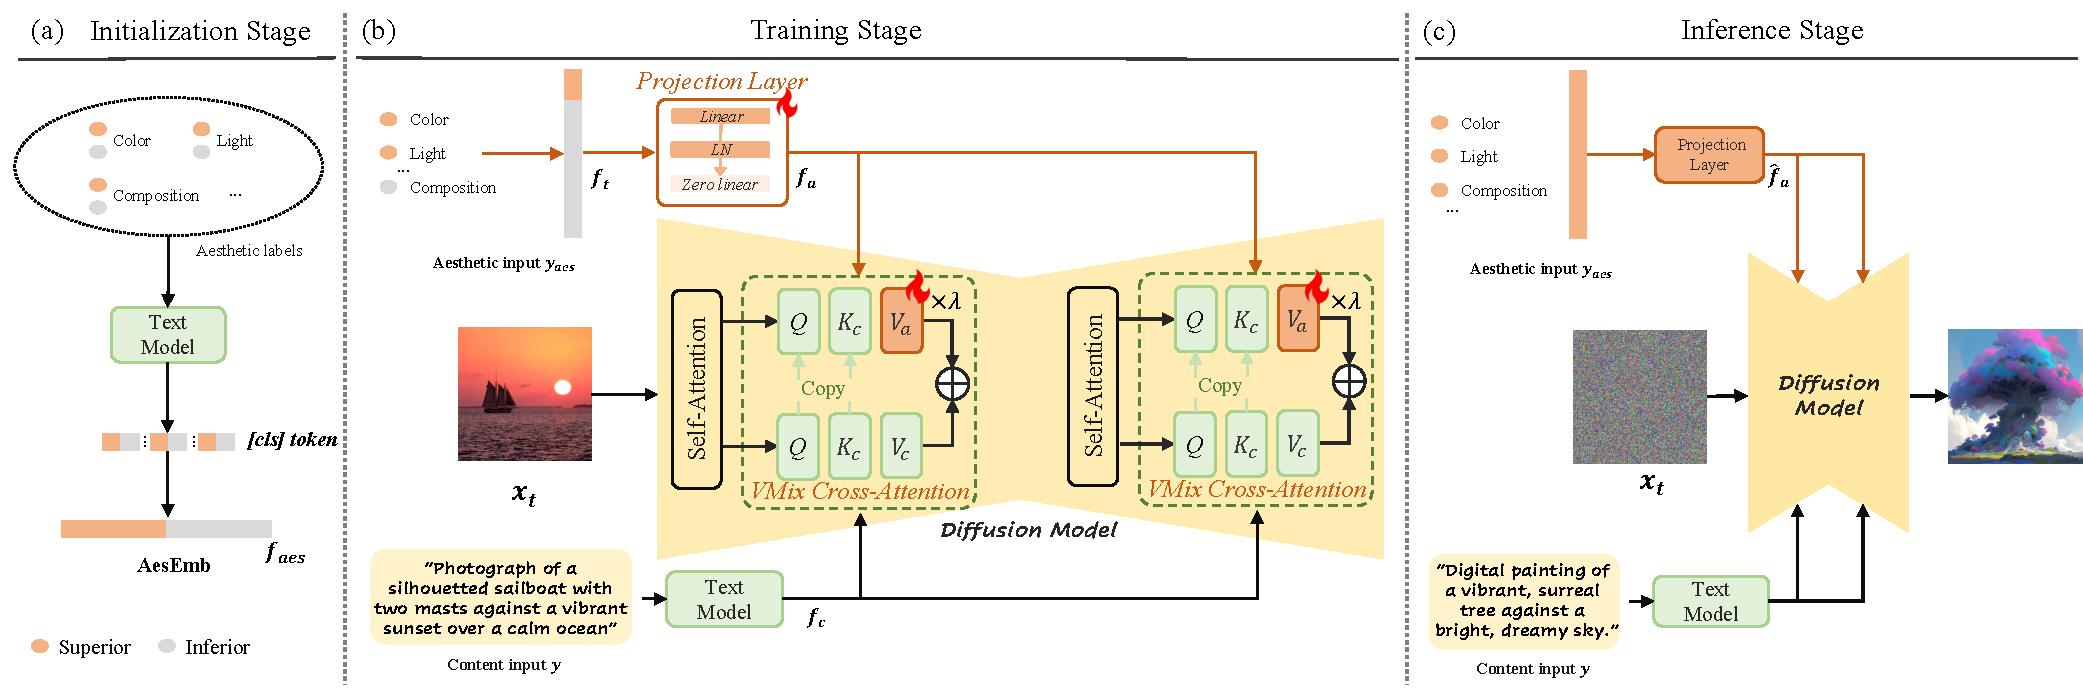
\includegraphics[scale=0.46]{overall_framework2.pdf}}
	\caption{Illustration of of VMix. (a)In the initialization stage, pre-defined aesthetic labels are transformed into [CLS] tokens through CLIP, thereby obtaining AesEmb, which only need to be processed once at the beginning of training. (b)In the training stage, a project layer first maps the input aesthetic description $y_{aes}$ into an embedding $f_a$ of the same token dimension as the content text embedding $f_t$. The text embedding $f_t$ is then integrated into the denoising network through value-mixed cross-attention. (c)In the inference stage, VMix extract all positive aesthetic embedding from AesEmb to form the aesthetic input, along with the content input, is fed into the model for the denoising process.}
	\label{Figure 1}
\end{figure*}


\subsection{Controlling Text-to-Image Models} 
Text-to-image models can generate results that match specific tasks or personalized content or styles by incorporating additional controlling conditions~\cite{mou2023t2i,wei2023elite}. Diverse conditional control approaches typically vary in the specific conditional features they introduce or the distinct points at which these conditions are injected into the process. ControlNet~\cite{zhang2023adding} integrates additional features into the decoder of the U-Net architecture to learn task-specific input conditions, such as pose, edges, sketch, and depth etc.\ IP-Adapter~\cite{ye2023ip} propose a unique decoupled cross-attention design for controllable image generation. Differing from these approaches, our method does not rely on reference images; instead, it disentangles the input text prompt into content description and aesthetic description and introduces distinctive improvements to the cross-attention layers.

% \begin{figure}[h]
% \centering
% 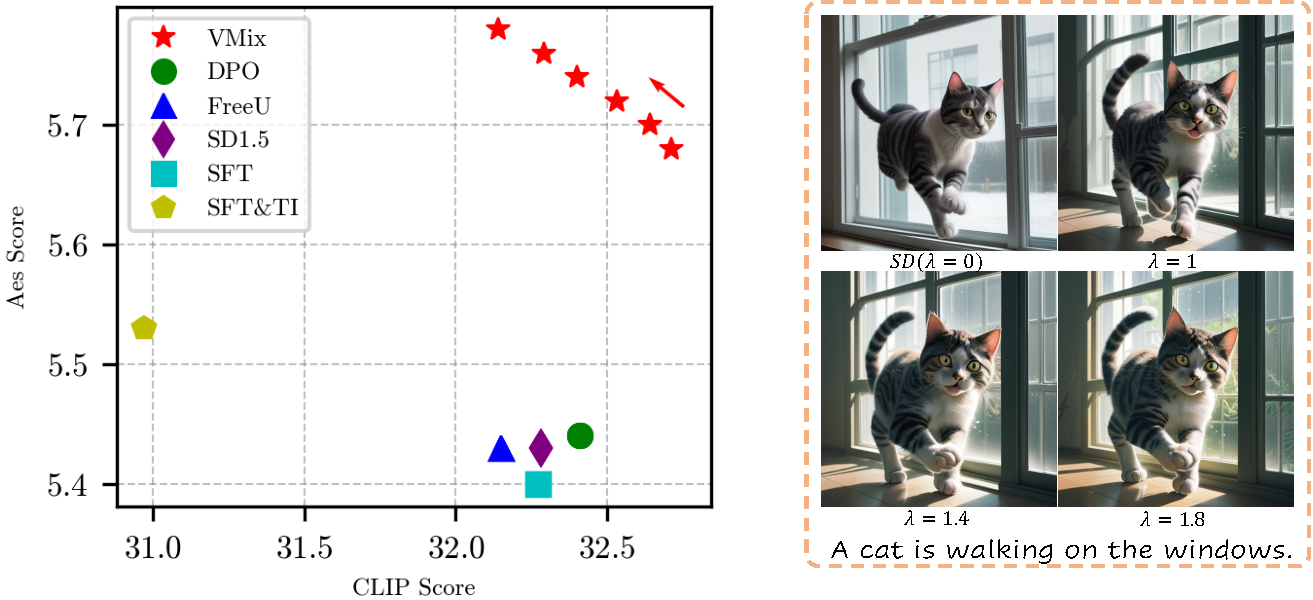
\includegraphics[scale=0.5]{lambd_fig2.pdf}
%     \caption{ Adaptation of $\lambda$. Prompts: (1) A boy, sitting in a tree, taking a nap, the shade of the tree, the afternoon sun shining through the leaves on the boy’s face, bust. (2) A cat is running on the windows.}
%     \label{Figure 2}
% \end{figure}